\documentclass[a4paper,12pt]{article} 

% First, we usually want to set the margins of our document. For this we use the package geometry.
\usepackage[top = 2.5cm, bottom = 2.5cm, left = 2.5cm, right = 2.5cm]{geometry} 
\usepackage[T1]{fontenc}
\usepackage[utf8]{inputenc}

% The following two packages - multirow and booktabs - are needed to create nice looking tables.
\usepackage{multirow} % Multirow is for tables with multiple rows within one cell.
\usepackage{booktabs} % For even nicer tables.

% As we usually want to include some plots (.pdf files) we need a package for that.
\usepackage{graphicx} 

% The default setting of LaTeX is to indent new paragraphs. This is useful for articles. But not really nice for homework problem sets. The following command sets the indent to 0.
%\usepackage{setspace}
%\setlength{\parindent}{0in}
\usepackage{indentfirst}

% Package to place figures where you want them.
\usepackage{float}

% The fancyhdr package let's us create nice headers.
\usepackage{fancyhdr}

\usepackage{amsmath,amsthm,karnaugh-map,caption,circuitikz}

\usepackage{tikz}
\usetikzlibrary{automata,positioning,patterns}

% To make our document nice we want a header and number the pages in the footer.

\pagestyle{fancy} % With this command we can customize the header style.

\fancyhf{} % This makes sure we do not have other information in our header or footer.

\lhead{\footnotesize Digital Logic(H): Theory Assignment 3}% \lhead puts text in the top left corner. \footnotesize sets our font to a smaller size.

%\rhead works just like \lhead (you can also use \chead)
\rhead{\footnotesize Mengxuan Wu} %<---- Fill in your lastnames.

% Similar commands work for the footer (\lfoot, \cfoot and \rfoot).
% We want to put our page number in the center.
\cfoot{\footnotesize \thepage} 

\begin{document}

\thispagestyle{empty} % This command disables the header on the first page. 

\begin{tabular}{p{15.5cm}}
{\large \bf Digital Logic(H)} \\
Southern University of Science and Technology \\ Mengxuan Wu \\ 12212006 \\
\hline
\\
\end{tabular}

\vspace*{0.3cm} %add some vertical space in between the line and our title.

\begin{center}
	{\Large \bf Theory Assignment 3}
	\vspace{2mm}

	{\bf Mengxuan Wu}
		
\end{center}  

\vspace{0.4cm}

\section*{1.}

\textbf{State Equation:}
\begin{align*}
	A(t+1) =& J_A A' + K_A' A = (Bx + B'y')A' + (B'xy')'A \\
	B(t+1) =& J_B B' + K_B' B = (A'x)B' + (A + xy')'B 
\end{align*}

\textbf{Output Equation: }
\begin{align*}
	z =& Ax'y' + Bx'y'
\end{align*}

\textbf{State Table:}
\begin{center}
	\begin{tabular}{ccccccc}
		\toprule
		\multicolumn{2}{c}{Present State} & \multicolumn{2}{c}{Input} & \multicolumn{2}{c}{Next State} & Output \\
		\cmidrule(lr){1-2} \cmidrule(lr){3-4} \cmidrule(lr){5-6} \cmidrule(lr){7-7}
		$A$ & $B$ & $x$ & $y$ & $A$ & $B$ & $z$ \\
		\midrule
		0 & 0 & 0 & 0 & 1 & 0 & 0 \\
		0 & 0 & 0 & 1 & 0 & 0 & 0 \\
		0 & 0 & 1 & 0 & 1 & 1 & 0 \\
		0 & 0 & 1 & 1 & 0 & 1 & 0 \\
		0 & 1 & 0 & 0 & 0 & 1 & 1 \\
		0 & 1 & 0 & 1 & 0 & 1 & 0 \\
		0 & 1 & 1 & 0 & 1 & 0 & 0 \\
		0 & 1 & 1 & 1 & 1 & 1 & 0 \\
		1 & 0 & 0 & 0 & 1 & 0 & 1 \\
		1 & 0 & 0 & 1 & 1 & 0 & 0 \\
		1 & 0 & 1 & 0 & 0 & 0 & 0 \\
		1 & 0 & 1 & 1 & 1 & 0 & 0 \\
		1 & 1 & 0 & 0 & 1 & 0 & 1 \\
		1 & 1 & 0 & 1 & 1 & 0 & 0 \\
		1 & 1 & 1 & 0 & 1 & 0 & 0 \\
		1 & 1 & 1 & 1 & 1 & 0 & 0 \\
		\bottomrule
	\end{tabular}
\end{center}

\newpage
\textbf{State Diagram:}
\begin{center}
	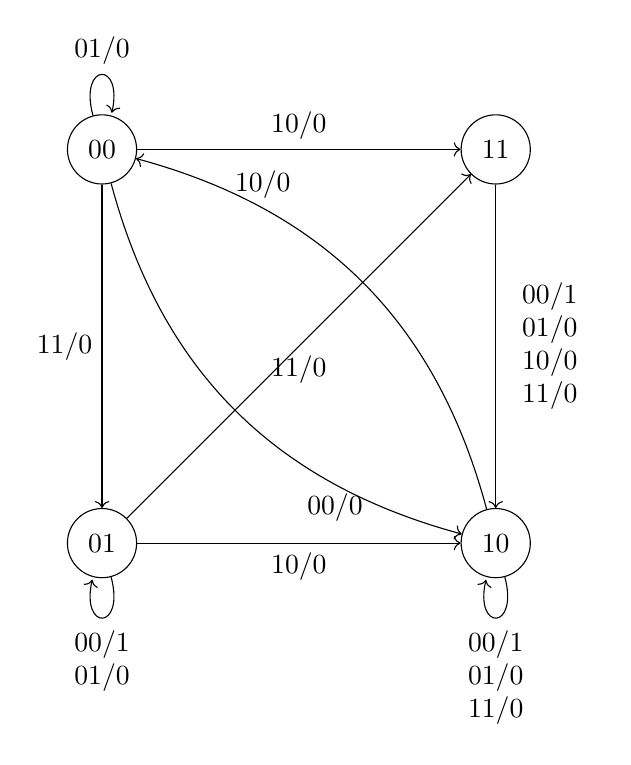
\begin{tikzpicture}[auto]
		\draw (0,0) node[state] (00) {00};
		\draw (0,-5) node[state] (01) {01};
		\draw (5,-5) node[state] (10) {10};
		\draw (5,0) node[state] (11) {11};

		\path[->]
			(00) edge [bend right]  node [near end, below]  	{00/0} 																(10)
			     edge [loop above]  node 						{01/0} 																(00)
				 edge               node 						{10/0}																(11)
				 edge 			    node [left]					{11/0} 																(01)
		    (01) edge [loop below]  node 						{\begin{tabular}{c} 00/1 \\ 01/0 \end{tabular}} 					(01)
			     edge 			    node [below] 				{10/0} 																(10)
				 edge 				node [below] 				{11/0} 																(11)
		    (10) edge [loop below]  node						{\begin{tabular}{c} 00/1 \\ 01/0 \\ 11/0 \end{tabular}} 			(10)
			     edge [bend right]  node [near end, above]   	{10/0} 																(00)
			(11) edge 				node [right] 				{\begin{tabular}{c} 00/1 \\ 01/0 \\ 10/0 \\ 11/0 \end{tabular}} 	(10);
		\end{tikzpicture}
\end{center}

\section*{2.}

\textbf{Input Equation:}

\begin{align*}
	T_A =& A + B \\
	T_B =& A' + B
\end{align*}

\textbf{Output Equation:}

\begin{align*}
	A(t+1) =& A \oplus T_A = A \oplus (A + B) \\
	B(t+1) =& B \oplus T_B = B \oplus (A' + B) 
\end{align*}

\textbf{State Table:}

\begin{center}
	\begin{tabular}{cccc}
		\toprule
		\multicolumn{2}{c}{Present State} & \multicolumn{2}{c}{Next State} \\
		\cmidrule(lr){1-2} \cmidrule(lr){3-4}
		$A$ & $B$ & $A$ & $B$ \\
		\midrule
		0 & 0 & 0 & 1 \\
		0 & 1 & 1 & 0 \\
		1 & 0 & 0 & 0 \\
		1 & 1 & 0 & 0 \\
		\bottomrule
	\end{tabular}
\end{center}
	
\newpage
\textbf{State Diagram:}

\begin{center}
	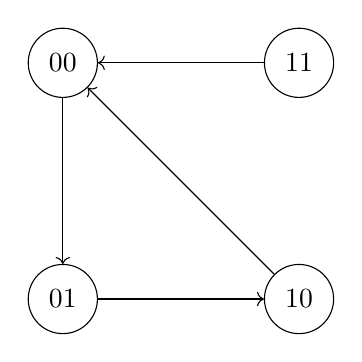
\begin{tikzpicture}[auto]
		\draw (0,0) node[state] (00) {00};
		\draw (0,-3) node[state] (01) {01};
		\draw (3,-3) node[state] (10) {10};
		\draw (3,0) node[state] (11) {11};

		\path[->]
			(00) edge (01)
			(01) edge (10)
			(10) edge (00)
			(11) edge (00)
			;
		\end{tikzpicture}
\end{center}

\section*{3.}

\subsection*{a)}

\textbf{Input Equation:}

\begin{align*}
	J_1 =& X   &K_1 = (XQ_2')' \\
	J_2 =& X   &K_2 = (XQ_1)'
\end{align*}

\textbf{State Equation:}

\begin{align*}
	Q_1(t+1) =& J_1Q_1' + K_1'Q_1 = XQ_1' + XQ_1Q_2' \\
	Q_2(t+1) =& J_2Q_2' + K_2'Q_2 = XQ_2' + XQ_1Q_2
\end{align*}

\textbf{Output Equation:}

\begin{equation*}
	F = X \oplus Q_2'
\end{equation*}

\textbf{State Table:}

\begin{center}
	\begin{tabular}{cccccc}
		\toprule
		\multicolumn{2}{c}{Present State} & Input & \multicolumn{2}{c}{Next State} & Output \\
		\cmidrule(lr){1-2} \cmidrule(lr){3-3} \cmidrule(lr){4-5} \cmidrule(lr){6-6}
		$Q_1$ & $Q_2$ & $X$ & $Q_1$ & $Q_2$ & $F$ \\
		\midrule
		0 & 0 & 0 & 0 & 0 & 1 \\
		0 & 0 & 1 & 1 & 1 & 0 \\
		0 & 1 & 0 & 0 & 0 & 0 \\
		0 & 1 & 1 & 1 & 0 & 1 \\
		1 & 0 & 0 & 0 & 0 & 1 \\
		1 & 0 & 1 & 1 & 1 & 0 \\
		1 & 1 & 0 & 0 & 0 & 0 \\
		1 & 1 & 1 & 0 & 1 & 1 \\
		\bottomrule
	\end{tabular}
\end{center}

\newpage
\textbf{State Diagram:}

\begin{center}
	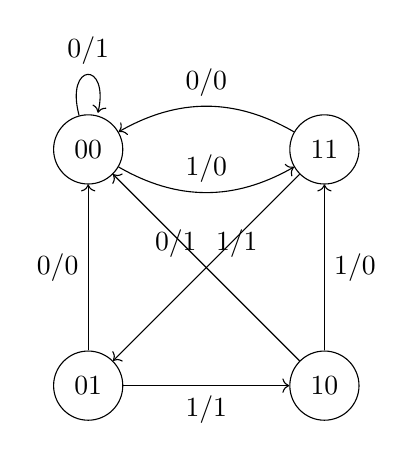
\begin{tikzpicture}[auto]
		\draw (0,0) node[state] (00) {00};
		\draw (0,-3) node[state] (01) {01};
		\draw (3,-3) node[state] (10) {10};
		\draw (3,0) node[state] (11) {11};

		\path[->]
			(00) 	edge	[loop above] 	node 					{0/1} 			(00)
				 	edge 	[bend right]	node 					{1/0} 			(11)
			(01) 	edge				 	node 					{0/0} 			(00)
					edge 					node 	[below]			{1/1} 			(10)
			(10) 	edge 					node 	[above left]	{0/1} 			(00)
					edge 					node 	[right]			{1/0} 			(11)
			(11) 	edge	[bend right] 	node 	[above]			{0/0} 			(00)
					edge 					node 	[above right]	{1/1} 			(01)
			;
	\end{tikzpicture}
\end{center}

\subsection*{b)}

This is a Mealy machine, because the output is determined by the input and the present state.
For example, when the present state is 00, the output is different when the input is 0 or 1.

\subsection*{c)}

\begin{center}
	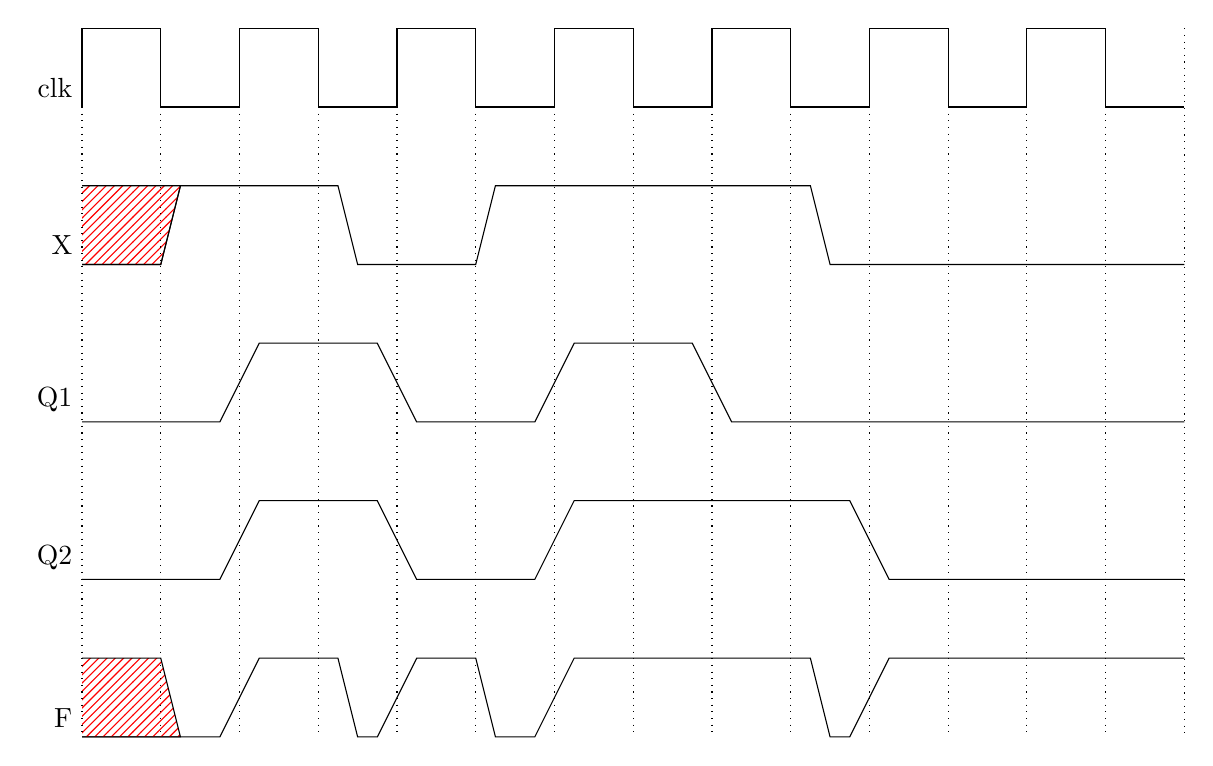
\begin{tikzpicture}
		\draw (0,0) node [above left] {clk} -- (0,1) -- (1,1) -- (1,0) -- (2,0) -- (2,1) -- (3,1) -- (3,0) -- (4,0) -- (4,1) -- (5,1) -- (5,0) -- (6,0) -- (6,1) -- (7,1) -- (7,0) -- (8,0) -- (8,1) -- (9,1) -- (9,0) -- (10,0) -- (10,1) -- (11,1) -- (11,0) -- (12,0) -- (12,1) -- (13,1) -- (13,0) -- (14,0);
		\draw (0,-2) node [above left] {X} -- (1,-2) -- (1.25,-1) -- (3.25,-1) -- (3.5,-2) -- (5,-2) -- (5.25,-1) -- (9.25,-1) -- (9.5,-2) -- (14,-2);
		\draw[pattern={north east lines},pattern color=red]  (0,-2) -- (1,-2) -- (1.25,-1) -- (0,-1);
		\draw (0,-4) node [above left] {Q1} -- (1.75,-4) -- (2.25,-3) -- (3.75,-3) -- (4.25,-4) -- (5.75,-4) -- (6.25,-3) -- (7.75,-3) -- (8.25,-4) -- (14,-4);
		\draw (0,-6) node [above left] {Q2} -- (1.75,-6) -- (2.25,-5) -- (3.75,-5) -- (4.25,-6) -- (5.75,-6) -- (6.25,-5) -- (9.75,-5) -- (10.25,-6) -- (14,-6);
		\draw (0,-8) node [above left] {F} -- (1.75,-8) -- (2.25,-7) -- (3.25,-7) -- (3.5,-8) -- (3.75,-8) -- (4.25,-7) -- (5,-7) -- (5.25,-8) -- (5.75,-8) -- (6.25,-7) -- (9.25,-7) -- (9.5,-8) -- (9.75,-8) -- (10.25,-7) -- (14,-7);
		\draw[pattern={north east lines},pattern color=red]  (0,-7) -- (1,-7) -- (1.25,-8) -- (0,-8); 
		\draw[dotted] (0,0) -- (0,-8);
		\draw[dotted] (1,0) -- (1,-8);
		\draw[dotted] (2,0) -- (2,-8);
		\draw[dotted] (3,0) -- (3,-8);
		\draw[dotted] (4,0) -- (4,-8);
		\draw[dotted] (5,0) -- (5,-8);
		\draw[dotted] (6,0) -- (6,-8);
		\draw[dotted] (7,0) -- (7,-8);
		\draw[dotted] (8,0) -- (8,-8);
		\draw[dotted] (9,0) -- (9,-8);
		\draw[dotted] (10,0) -- (10,-8);
		\draw[dotted] (11,0) -- (11,-8);
		\draw[dotted] (12,0) -- (12,-8);
		\draw[dotted] (13,0) -- (13,-8);
		\draw[dotted] (14,1) -- (14,-8);
	\end{tikzpicture}
\end{center}

\newpage
\section*{4.}

\textbf{State Table:}

\begin{center}
	\begin{tabular}{ccccc}
		\toprule
		Present State & Input & Next State \\
		\cmidrule(lr){1-1} \cmidrule(lr){2-2} \cmidrule(lr){3-3}
		$Q$ & $X$ & $Q$ \\
		\midrule
		$a$ & 0 & $b$ \\
		$a$ & 1 & $a$ \\
		$b$ & 0 & $d$ \\
		$b$ & 1 & $c$ \\
		$c$ & 0 & $d$ \\
		$c$ & 1 & $c$ \\
		$d$ & 0 & $a$ \\
		$d$ & 1 & $d$ \\
		\bottomrule
	\end{tabular}
\end{center}

\textbf{Reduced State Table:}

\begin{center}
	\begin{tabular}{ccccc}
		\toprule
		Present State & Input & Next State \\
		\cmidrule(lr){1-1} \cmidrule(lr){2-2} \cmidrule(lr){3-3}
		$Q$ & $X$ & $Q$ \\
		\midrule
		$a$ & 0 & $b$ \\
		$a$ & 1 & $a$ \\
		$b$ & 0 & $d$ \\
		$b$ & 1 & $b$ \\
		$d$ & 0 & $a$ \\
		$d$ & 1 & $d$ \\
		\bottomrule
	\end{tabular}
\end{center}

Let $a = 00$, $b = 01$, $d = 10$, then the reduced state table is:
\textbf{State Table with TFF Input:}

\begin{center}
	\begin{tabular}{ccccccc}
		\toprule
		\multicolumn{2}{c}{Present State} & Input & \multicolumn{2}{c}{Next State} & \multicolumn{2}{c}{TFF Input} \\
		\cmidrule(lr){1-2} \cmidrule(lr){3-3} \cmidrule(lr){4-5} \cmidrule(lr){6-7}
		$Q_1$ & $Q_2$ & $X$ & $Q_1$ & $Q_2$ & $T_1$ & $T_2$ \\
		\midrule
		0 & 0 & 0 & 0 & 1 & 0 & 1 \\
		0 & 0 & 1 & 0 & 0 & 0 & 0 \\
		0 & 1 & 0 & 1 & 0 & 1 & 1 \\
		0 & 1 & 1 & 0 & 1 & 0 & 0 \\
		1 & 0 & 0 & 0 & 0 & 1 & 0 \\
		1 & 0 & 1 & 1 & 0 & 0 & 0 \\
		1 & 1 & 0 & X & X & X & X \\
		1 & 1 & 1 & X & X & X & X \\
		\bottomrule
	\end{tabular}
\end{center}

\newpage
\textbf{Derive Input Equation:}

\begin{figure}[H]
	\begin{minipage}{0.5\linewidth}
		\centering
		\begin{karnaugh-map}(label=corner)[4][2][1][$Q_2X$][$Q_1$]
			\minterms{2,4}
			\maxterms{0,1,3,5}
			\autoterms[X]
			\implicant{2}{6}
			\implicantedge{4}{4}{6}{6}
		\end{karnaugh-map}
		\caption*{$T_1$}
	\end{minipage}
	\begin{minipage}{0.5\linewidth}
		\centering
		\begin{karnaugh-map}(label=corner)[4][2][1][$Q_2X$][$Q_1$]
			\minterms{0,2}
			\maxterms{1,3,4,5}
			\autoterms[X]
			\implicantedge{0}{0}{2}{2}
		\end{karnaugh-map}
		\caption*{$T_2$}
	\end{minipage}
\end{figure}

\begin{align*}
	T_1 =& Q_1X' + Q_2X' \\
	T_2 =& Q_1'X'
\end{align*}

\section*{5.}

\textbf{State Table:}

\begin{center}
	\begin{tabular}{cccc}
		\toprule
		Present State & \multicolumn{2}{c}{Input} & Next State \\
		\cmidrule(lr){1-1} \cmidrule(lr){2-3} \cmidrule(lr){4-4}
		$Q$ & $En$ & $D$ & $Q$ \\
		\midrule
		0 & 0 & 0 & 0 \\
		0 & 0 & 1 & 0 \\
		0 & 1 & 0 & 0 \\
		0 & 1 & 1 & 1 \\
		1 & 0 & 0 & 1 \\
		1 & 0 & 1 & 1 \\
		1 & 1 & 0 & 0 \\
		1 & 1 & 1 & 1 \\
		\bottomrule
	\end{tabular}
\end{center}

\textbf{Derive Input Equation:}

\begin{center}
	\begin{karnaugh-map}(label=corner)[4][2][1][$En D$][$Q$]
		\minterms{3,4,5,7}
		\autoterms[0]
		\implicant{3}{7}
		\implicant{4}{5}
	\end{karnaugh-map}
\end{center}

\begin{equation*}
	Q(t+1) = EnD + QEn'
\end{equation*}

\newpage
\textbf{Block Diagram:}

\begin{center}
	\begin{circuitikz}
		\tikzset{myflipflop D/.style={flipflop,flipflop def={t1=D, t3={\texttt{CLK}}, t4=Q, t6=Q, n4=1, c3=1}}}
		\draw 
			(0,0) 		node [myflipflop D]				(DFF)	{}
			(-9,0) 		node [left]						(En)	{$En$}
			(-9,-1) 	node [left]						(D)		{$D$}
			(-7,0)  	node [not port, scale = 0.3]	(En')	{}
			(-6,-0.8)	node [and port, scale = 0.8]	(and1)	{}
			(-5,0.8) 	node [and port, scale = 0.8]	(and2)	{}
			(-2,0.85) 	node [or port, scale = 0.8]		(or)	{};

		\draw 
			(En) -- (En'.in)
			(En) -- ++(1,0) node [circ] (divert1) {} -- (divert1 |- and1.in 1) -- (and1.in 1)
			(D) -- (and1.in 2)
			(En'.out) -- ++(0.5,0) |- (and2.in 2)
			(DFF.pin 6) -- ++(0.3,0) -- ++(0,1) -| (and2.in 1)
			(and2.out) -- ++(0.5,0) |- (or.in 1)
			(and1.out) -| (or.in 2)
			(or.out) -- (DFF.pin 1)
			(DFF.pin 3) -- ++(-0.3,0) -- ++(0,-1) node [below] {$clk$}
			;
	\end{circuitikz}
\end{center}

\section*{6.}

\subsection*{a)}

\textbf{Characteristic Table:}

\begin{center}
	\begin{tabular}{cccc}
		\toprule
		$A$ & $B$ & $Q(t+1)$ & Operation \\
		\midrule
		0 & 0 & 0 & Reset \\
		0 & 1 & $Q(t)$ & No Change \\
		1 & 0 & $Q(t)'$ & Complement \\
		1 & 1 & 1 & Set \\
		\bottomrule
	\end{tabular}
\end{center}

\subsection*{b)}

\textbf{Characteristic Equation:}

\begin{equation*}
	Q(t+1) = A'BQ + AB'Q' + AB
\end{equation*}

\textbf{State Table:}

\begin{center}
	\begin{tabular}{cccc}
		\toprule
		Current State & \multicolumn{2}{c}{Input} & Next State \\
		\cmidrule(lr){1-1} \cmidrule(lr){2-3} \cmidrule(lr){4-4}
		$Q$ & $A$ & $B$ & $Q$ \\
		\midrule
		0 & 0 & 0 & 0 \\
		0 & 0 & 1 & 0 \\
		0 & 1 & 0 & 1 \\
		0 & 1 & 1 & 1 \\
		1 & 0 & 0 & 0 \\
		1 & 0 & 1 & 1 \\
		1 & 1 & 0 & 0 \\
		1 & 1 & 1 & 1 \\
		\bottomrule
	\end{tabular}
\end{center}

\newpage
\textbf{Simplify Characteristic Equation:}

\begin{center}
	\begin{karnaugh-map}(label=corner)[4][2][1][$AB$][$Q$]
		\minterms{2,3,5,7}
		\autoterms[0]
		\implicant{3}{2}
		\implicant{5}{7}
	\end{karnaugh-map}
\end{center}

\begin{equation*}
	Q(t+1) = Q'A + QB
\end{equation*}

\subsection*{c)}

\textbf{Excitation Table:}

\begin{center}
	\begin{tabular}{ccccc}
		\toprule
		$Q(t)$ & $Q(t+1)$ & $A$ & $B$ & Operation \\
		\midrule
		0 & 0 & 0 & X & Reset \\
		0 & 1 & 1 & X & No Change \\
		1 & 0 & X & 0 & Complement \\
		1 & 1 & X & 1 & Set \\
		\bottomrule
	\end{tabular}
\end{center}

\subsection*{d)}

\textbf{State Table with JKFF Input:}

\begin{center}
	\begin{tabular}{cccccc}
		\toprule
		Current State & \multicolumn{2}{c}{JKFF Input} & Next State & \multicolumn{2}{c}{New FF Input} \\
		\cmidrule(lr){1-1} \cmidrule(lr){2-3} \cmidrule(lr){4-4} \cmidrule(lr){5-6}
		$Q$ & $J$ & $K$ & $Q$ & $A$ & $B$ \\
		\midrule
		0 & 0 & 0 & 0 & 0 & X \\
		0 & 0 & 1 & 0 & 0 & X \\
		0 & 1 & 0 & 1 & 1 & X \\
		0 & 1 & 1 & 1 & 1 & X \\
		1 & 0 & 0 & 1 & X & 1 \\
		1 & 0 & 1 & 0 & X & 0 \\
		1 & 1 & 0 & 1 & X & 1 \\
		1 & 1 & 1 & 0 & X & 0 \\
		\bottomrule
	\end{tabular}
\end{center}

\textbf{Simplify New FF Input:}

\begin{figure}[H]
	\begin{minipage}{0.5\linewidth}
		\centering
		\begin{karnaugh-map}(label=corner)[4][2][1][$JK$][$Q$]
			\minterms{2,3}
			\maxterms{0,1}
			\autoterms[X]
			\implicant{3}{6}
		\end{karnaugh-map}
		\caption*{$A$}
	\end{minipage}
	\begin{minipage}{0.5\linewidth}
		\centering
		\begin{karnaugh-map}(label=corner)[4][2][1][$JK$][$Q$]
			\minterms{4,6}
			\maxterms{5,7}
			\autoterms[X]
			\implicantedge{0}{4}{2}{6}
		\end{karnaugh-map}
		\caption*{$B$}
	\end{minipage}
\end{figure}

The simplified JKFF input is:
\begin{align*}
	A =& J \\
	B =& K'
\end{align*}

\textbf{Block Diagram:}

\begin{center}
	\begin{circuitikz}
		\tikzset{myflipflop New/.style={flipflop,flipflop def={t1=A, t2={\texttt{CLK}}, t3=B, t4=Q, t6=Q, n4=1, c2=1}}}
		\draw 
			(0,0) 		node [myflipflop New]			(JKFF)	{}
			(-5,0.85) 	node [left]						(A)		{$J$}
			(-5,-0.85) 	node [left]						(B)		{$K$}
			(-4,-0.85)  	node [not port, scale = 0.3]	(B')	{}
			;
		\draw 
			(JKFF.pin 2) -- ++(-0.3,0) -- ++(0,-3) node [below] {$clk$}
			(B) -- (B'.in)
			(A) -- (JKFF.pin 1)
			(B'.out) -- (JKFF.pin 3)
			;
	\end{circuitikz}
\end{center}

\section*{7.}

\textbf{Reduced State Table:}

\begin{center}
	\begin{tabular}{ccccc}
		\toprule
		\multirow{2}{*}{Present State} & \multicolumn{2}{c}{Next State} & \multicolumn{2}{c}{Output} \\
		\cmidrule(lr){2-3} \cmidrule(lr){4-5}
		& $X = 0$ & $X = 1$ & $X = 0$ & $X = 1$ \\
		\midrule
		$a$ & $f$ & $b$ & 0 & 0 \\
		$b$ & $d$ & $a$ & 0 & 0 \\
		$d$ & $g$ & $a$ & 1 & 0 \\
		$f$ & $f$ & $b$ & 1 & 1 \\
		$g$ & $g$ & $d$ & 0 & 1 \\
		\bottomrule
	\end{tabular}
\end{center}

\textbf{State Diagram:}

\begin{center}
	\begin{tikzpicture}[auto]
		\draw 
			(0,0) node [state] (a) {$a$}
			(-2,-4) node [state] (b) {$b$}
			(4,-7) node [state] (d) {$d$}
			(10,-4) node [state] (f) {$f$}
			(8,0) node [state] (g) {$g$}
			;
		\draw[->]
			(a) edge [near start] node {0/0} (f)
			    edge [bend right] node [left] {1/0} (b)
			(b) edge node [below] {0/0} (d)
				edge [bend right] node {1/0} (a)
			(d) edge [near start, bend right] node [below right] {0/1} (g)
				edge [near start] node {1/0} (a)
			(f) edge [loop below] node {0/1} (f)
				edge [near end] node {1/1} (b)
			(g) edge [loop above] node {0/0} (g)
				edge [near start, bend right] node [above] {1/1} (d)
			;
	\end{tikzpicture}
\end{center}

\newpage
Let $a = 000$, $b = 001$, $d = 010$, $f = 011$, $g = 100$.

\textbf{State Table with JKFF Input:}

\begin{center}
	\begin{tabular}{cccccccccccccc}
		\toprule
		\multicolumn{3}{c}{Present State} & Input & \multicolumn{3}{c}{Next State} & \multicolumn{6}{c}{JKFF Input} & Output \\
		\cmidrule(lr){1-3} \cmidrule(lr){4-4} \cmidrule(lr){5-7} \cmidrule(lr){8-13} \cmidrule(lr){14-14}
		$Q_1$ & $Q_2$ & $Q_3$ & $X$ & $Q_1$ & $Q_2$ & $Q_3$ & $J_1$ & $K_1$ & $J_2$ & $K_2$ & $J_3$ & $K_3$ & $F$ \\
		\midrule
		0 & 0 & 0 & 0 & 0 & 1 & 1 & 0 & X & 1 & X & 1 & X & 0 \\
		0 & 0 & 0 & 1 & 0 & 0 & 1 & 0 & X & 0 & X & 1 & X & 0 \\
		0 & 0 & 1 & 0 & 0 & 1 & 0 & 0 & X & 1 & X & X & 1 & 0 \\
		0 & 0 & 1 & 1 & 0 & 0 & 0 & 0 & X & 0 & X & X & 1 & 0 \\
		0 & 1 & 0 & 0 & 1 & 0 & 0 & 1 & X & X & 1 & 0 & X & 1 \\
		0 & 1 & 0 & 1 & 0 & 0 & 0 & 0 & X & X & 1 & 0 & X & 0 \\
		0 & 1 & 1 & 0 & 0 & 1 & 1 & 0 & X & X & 0 & X & 0 & 1 \\
		0 & 1 & 1 & 1 & 0 & 0 & 1 & 0 & X & X & 1 & X & 0 & 1 \\
		1 & 0 & 0 & 0 & 1 & 0 & 0 & X & 0 & 0 & X & 0 & X & 0 \\
		1 & 0 & 0 & 1 & 0 & 1 & 0 & X & 1 & 1 & X & 0 & X & 1 \\
		1 & 0 & 1 & 0 & X & X & X & X & X & X & X & X & X & X \\
		1 & 0 & 1 & 1 & X & X & X & X & X & X & X & X & X & X \\
		1 & 1 & 0 & 0 & X & X & X & X & X & X & X & X & X & X \\
		1 & 1 & 0 & 1 & X & X & X & X & X & X & X & X & X & X \\
		1 & 1 & 1 & 0 & X & X & X & X & X & X & X & X & X & X \\
		1 & 1 & 1 & 1 & X & X & X & X & X & X & X & X & X & X \\
		\bottomrule
	\end{tabular}
\end{center}

\textbf{Simplify JKFF Input:}

\begin{figure}[H]
	\begin{minipage}{0.5\linewidth}
		\centering
		\begin{karnaugh-map}(label=corner)[4][4][1][$Q_3X$][$Q_1Q_2$]
			\minterms{4}
			\maxterms{0,1,2,3,5,6,7}
			\autoterms[X]
			\implicant{4}{12}
		\end{karnaugh-map}
		\caption*{$J_1$}
	\end{minipage}
	\begin{minipage}{0.5\linewidth}
		\centering
		\begin{karnaugh-map}(label=corner)[4][4][1][$Q_3X$][$Q_1Q_2$]
			\minterms{9}
			\maxterms{8}
			\autoterms[X]
			\implicant{1}{11}
		\end{karnaugh-map}
		\caption*{$K_1$}
	\end{minipage}
\end{figure}

\begin{figure}[H]
	\begin{minipage}{0.5\linewidth}
		\centering
		\begin{karnaugh-map}(label=corner)[4][4][1][$Q_3X$][$Q_1Q_2$]
			\minterms{0,2,9}
			\maxterms{1,3,8}
			\autoterms[X]
			\implicant{13}{11}
			\implicantedge{0}{4}{2}{6}
		\end{karnaugh-map}
		\caption*{$J_2$}
	\end{minipage}
	\begin{minipage}{0.5\linewidth}
		\centering
		\begin{karnaugh-map}(label=corner)[4][4][1][$Q_3X$][$Q_1Q_2$]
			\minterms{4,5,7}
			\maxterms{6}
			\autoterms[X]
			\implicant{0}{9}
			\implicant{1}{11}
		\end{karnaugh-map}
		\caption*{$K_2$}
	\end{minipage}
\end{figure}

\begin{figure}[H]
	\begin{minipage}{0.5\linewidth}
		\centering
		\begin{karnaugh-map}(label=corner)[4][4][1][$Q_3X$][$Q_1Q_2$]
			\minterms{0,1}
			\maxterms{4,5,8,9}
			\autoterms[X]
			\implicant{0}{2}
		\end{karnaugh-map}
		\caption*{$J_3$}
	\end{minipage}
	\begin{minipage}{0.5\linewidth}
		\centering
		\begin{karnaugh-map}(label=corner)[4][4][1][$Q_3X$][$Q_1Q_2$]
			\minterms{2,3}
			\maxterms{6,7}
			\autoterms[X]
			\implicantedge{0}{2}{8}{10}
		\end{karnaugh-map}
		\caption*{$K_3$}
	\end{minipage}
\end{figure}

The simplified JKFF input is:
\begin{align*}
	J_1 =& Q_2Q_3'X' &K_1 =& X \\
	J_2 =& Q_1'X' + Q_1X &K_2 =& Q_3' + X \\
	J_3 =& Q_1'Q_2' &K_3 =& Q_2'
\end{align*}

\newpage
\section*{8.}

\textbf{State Diagram:}

\begin{center}
	\begin{tikzpicture}[auto]
		\draw 
			(0,0) node [state] (a) {$a/0$}
			(-2,-4) node [state] (b) {$b/0$}
			(4,-7) node [state] (c) {$c/0$}
			(10,-4) node [state] (d) {$d/0$}
			(8,0) node [state] (e) {$e/1$}
			;
		\draw[->]
			(a) edge [loop above] 	node 			{0} (a)
				edge [bend right]	node [left] 	{1} (b)
			(b) edge [bend right] 	node 		 	{0} (a)
				edge 				node [below] 	{1} (c)
			(c) edge 			 	node [below] 	{0} (d)
				edge [loop below]	node 		 	{1} (c)
			(d) edge 			 	node [above] 	{0} (a)
				edge 				node [above] 	{1} (e)
			(e) edge 			 	node [above]	{0} (a)
				edge 				node 		 	{1} (c)
			;
	\end{tikzpicture}
\end{center}

Let $a = 000$, $b = 001$, $c = 010$, $d = 011$, $e = 100$.

\textbf{State Table with DFF Input:}

\begin{center}
	\begin{tabular}{cccccccccc}
		\toprule
		\multicolumn{3}{c}{Present State} & Input & \multicolumn{3}{c}{Next State} & \multicolumn{3}{c}{DFF Input} \\
		\cmidrule(lr){1-3} \cmidrule(lr){4-4} \cmidrule(lr){5-7} \cmidrule(lr){8-10}
		$Q_1$ & $Q_2$ & $Q_3$ & $X$ & $Q_1$ & $Q_2$ & $Q_3$ & $D_1$ & $D_2$ & $D_3$ \\
		\midrule
		0 & 0 & 0 & 0 & 0 & 0 & 0 & 0 & 0 & 0 \\
		0 & 0 & 0 & 1 & 0 & 0 & 1 & 0 & 0 & 1 \\
		0 & 0 & 1 & 0 & 0 & 0 & 0 & 0 & 0 & 0 \\
		0 & 0 & 1 & 1 & 0 & 1 & 0 & 0 & 1 & 0 \\
		0 & 1 & 0 & 0 & 0 & 1 & 1 & 0 & 1 & 1 \\
		0 & 1 & 0 & 1 & 0 & 1 & 0 & 0 & 1 & 0 \\
		0 & 1 & 1 & 0 & 0 & 0 & 0 & 0 & 0 & 0 \\
		0 & 1 & 1 & 1 & 1 & 0 & 0 & 1 & 0 & 0 \\
		1 & 0 & 0 & 0 & 0 & 0 & 0 & 0 & 0 & 0 \\
		1 & 0 & 0 & 1 & 0 & 1 & 0 & 0 & 1 & 0 \\
		1 & 0 & 1 & 0 & X & X & X & X & X & X \\
		1 & 0 & 1 & 1 & X & X & X & X & X & X \\
		1 & 1 & 0 & 0 & X & X & X & X & X & X \\
		1 & 1 & 0 & 1 & X & X & X & X & X & X \\
		1 & 1 & 1 & 0 & X & X & X & X & X & X \\
		1 & 1 & 1 & 1 & X & X & X & X & X & X \\
		\bottomrule
	\end{tabular}
\end{center}

\newpage
\textbf{Simplify DFF Input:}

\begin{figure}[H]
	\begin{minipage}{0.32\linewidth}
		\centering
		\begin{karnaugh-map}(label=corner)[4][4][1][$Q_3X$][$Q_1Q_2$]
			\minterms{7}
			\maxterms{0,1,2,3,4,5,6,8,9}
			\autoterms[X]
			\implicant{7}{15}
		\end{karnaugh-map}
		\caption*{$D_1$}
	\end{minipage}
	\begin{minipage}{0.32\linewidth}
		\centering
		\begin{karnaugh-map}(label=corner)[4][4][1][$Q_3X$][$Q_1Q_2$]
			\minterms{3,4,5,9}
			\maxterms{0,1,2,6,7,8}
			\autoterms[X]
			\implicant{4}{13}
			\implicant{13}{11}
			\implicantedge{3}{3}{11}{11}
		\end{karnaugh-map}
		\caption*{$D_2$}
	\end{minipage}
	\begin{minipage}{0.32\linewidth}
		\centering
		\begin{karnaugh-map}(label=corner)[4][4][1][$Q_3X$][$Q_1Q_2$]
			\minterms{1,4}
			\maxterms{0,2,3,5,6,7,8,9}
			\autoterms[X]
			\implicant{1}{1}
			\implicant{4}{12}
		\end{karnaugh-map}
		\caption*{$D_3$}
	\end{minipage}
\end{figure}

The simplified DFF input is:
\begin{align*}
	D_1 =& Q_2Q_3X \\
	D_2 =& Q_2Q_3' + Q_1X + Q_2'Q_3X \\
	D_3 =& Q_2Q_3'X' + Q_1'Q_2'Q_3'X 
\end{align*}
\end{document}